\documentclass[10pt,a4paper]{article}

\usepackage[T1]{fontenc}
\usepackage[utf8]{inputenc}
\usepackage{lmodern}
\usepackage[margin=2.0cm]{geometry}
\usepackage{microtype}
\usepackage{booktabs}
\usepackage{graphicx}
\usepackage{xcolor}
\usepackage{tikz}
\usetikzlibrary{arrows.meta,positioning,calc}
\usepackage{enumitem}
\usepackage[font=small,labelfont=bf,skip=3pt]{caption}
\usepackage[colorlinks=true,linkcolor=blue!50!black,urlcolor=blue!50!black,citecolor=blue!50!black]{hyperref}
\usepackage{float}
\usepackage{xurl}
\emergencystretch=2em

\setlist{nosep,leftmargin=1.3em}
\setlength{\parskip}{0.3em}
\setlength{\parindent}{0pt}
\renewcommand{\arraystretch}{1.1}

\newcommand{\simd}[1]{\texttt{simd\_#1}}

\title{\bfseries A custom 4-lane INT8 multiply-accumulate instruction\\for a RISC-V core: design, verification and\\cycle-level measurement}
\author{Mir Mohammad Sajedul Islam\\[2pt]\small\href{mailto:sajedulislam5840@gmail.com}{sajedulislam5840@gmail.com}}
\date{}

\begin{document}
\maketitle

\begin{abstract}
\noindent Small, low-cost processors usually have no floating-point unit, yet we keep asking them to recognise images. I gave a RISC-V core one new instruction that does four 8-bit multiplications and adds the results in a single step. A handwritten-digit network that needed 2.58 million clock cycles now needs 0.58 million: \textbf{4.5$\times$ fewer cycles} at the same 98.2\% accuracy. The new hardware slows the clock by 14\%, so on an FPGA the real gain in time is \textbf{3.8$\times$}, for 419 LUT4 and 4 DSP blocks. The comparison is against an equally optimised scalar program, not a deliberately slow one. All results come from cycle-accurate simulation and synthesis, not from silicon; each can be reproduced from the public repository and is checked against a reference model.
\end{abstract}

\section{Introduction}
Cheap microcontrollers that have no floating-point unit can still run neural networks if the network uses integer arithmetic. A 32-bit RISC-V register holds four 8-bit values, but the base multiply instruction works on one pair at a time. A custom instruction that multiplies four pairs and adds the products is an obvious fit.

The idea is not new. Packed 8-bit multiply-accumulate instructions appear in the draft RISC-V P extension, and Arm's CMSIS-NN shows what optimised software can do on an existing microcontroller. This report makes no claim of a new instruction. Its contribution is a complete and reproducible path from a trained network to measured clock cycles, with a fair baseline and enough verification to trust the numbers:

\begin{itemize}
\item an integer-only INT8 quantisation scheme and a freestanding C firmware that runs the network on RV32IM;
\item a 4-lane MAC unit in Verilog with four instructions in the \texttt{custom-0} opcode, including a form that needs only two register read ports;
\item verification against a golden model, with checks that are shown to fail when the hardware is broken;
\item cycle-accurate measurement on PicoRV32 (cycles, memory wait states, area, clock speed), and a per-instruction trace of one neuron that shows where the cycles go.
\end{itemize}

\section{Background and related work}
\textbf{Integer-only quantisation.} Jacob et al.\ \cite{jacob2018} describe an affine INT8 scheme in which inference uses integer arithmetic only: a layer accumulates in INT32 and rescales with a fixed-point multiplier and shift. My runtime follows the same structure.

\textbf{Optimised software.} CMSIS-NN \cite{lai2018} provides hand-optimised kernels for Arm Cortex-M cores and reports a 4.6$\times$ gain in runtime on a CIFAR-10 network over its baseline. It is a software result on existing instructions and is not comparable with the numbers here.

\textbf{Packed SIMD in RISC-V.} The draft P extension proposes packed-SIMD instructions, including multiply-accumulate on packed subwords \cite{hauser}. It is a draft and not an official specification. I did not implement it and did not compare against it. My instruction is chosen for what a PicoRV32 coprocessor port can carry.

\textbf{Custom function units on soft cores.} CFU Playground \cite{prakash2023} is an open framework for designing accelerators that are coupled to a soft CPU on an FPGA, and it reports speed-ups of 55$\times$ to 75$\times$ on its own tinyML workloads. Those workloads, cores and accelerators differ from mine, so I report my own measurements only.

\textbf{Core.} PicoRV32 \cite{picorv32} is a small RV32IMC core with a coprocessor interface (PCPI). I use it with the fast multiplier, divider and barrel shifter, and without caches.

\section{Design}
\subsection{Quantised network}
The network is a 784-128-10 MLP trained in NumPy. Values are quantised as $q=\mathrm{clamp}(\mathrm{round}(r/S)+Z,-128,127)$. Weights are symmetric ($Z_W=0$), activations are asymmetric, and each layer is requantised with a Q31 multiplier and a shift, so inference has no floating-point operation. One inference takes 101,632 multiply-accumulates (784$\times$128 + 128$\times$10). INT8 weights need 101.6~KB, against 406.4~KB in FP32.

A layer needs $\sum_j (q_{x,j}-Z_x)\,w_j$, but the MAC unit multiplies raw signed bytes. Because the weights are symmetric, this splits into $\sum_j q_{x,j}w_j - Z_x\sum_j w_j$. The first sum is what the instruction computes. The second is a constant per output neuron and is folded into the bias offline. The test-vector generator checks this identity for every neuron.

\begin{figure}[htbp]
\centering
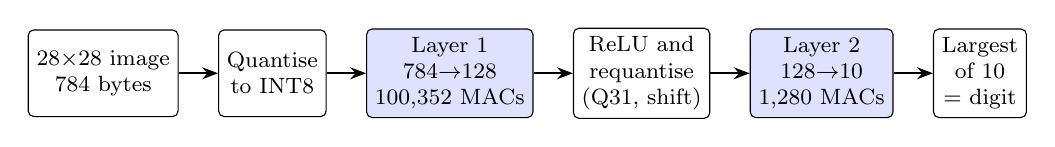
\begin{tikzpicture}[font=\footnotesize,node distance=5mm,
  blk/.style={draw,rounded corners=2pt,minimum height=11mm,align=center,inner sep=3pt},
  mac/.style={blk,fill=blue!12},
  arr/.style={-{Stealth[length=2mm]},thick}]
\node[blk] (img) {28$\times$28 image\\784 bytes};
\node[blk,right=of img] (q) {Quantise\\to INT8};
\node[mac,right=of q] (l1) {Layer 1\\784$\to$128\\100,352 MACs};
\node[blk,right=of l1] (r) {ReLU and\\requantise\\(Q31, shift)};
\node[mac,right=of r] (l2) {Layer 2\\128$\to$10\\1,280 MACs};
\node[blk,right=of l2] (am) {Largest\\of 10\\= digit};
\foreach \a/\b in {img/q,q/l1,l1/r,r/l2,l2/am} \draw[arr] (\a) -- (\b);
\end{tikzpicture}
\caption{The network as the firmware runs it. Only the two shaded layers use the custom instruction; everything else is integer arithmetic on a plain RV32IM core.}
\label{fig:pipeline}
\end{figure}

\subsection{The MAC unit and its instructions}
The unit (Figure~\ref{fig:datapath}) takes two 32-bit registers that each hold four signed INT8 values and computes
\[
\mathit{result} = (\mathit{clear}\;?\;0 : \mathit{total}) + a_0b_0 + a_1b_1 + a_2b_2 + a_3b_3
\]
in one clock cycle. Each product is at most $2^{14}$ in magnitude, so four products fit in 18 bits and only the 32-bit accumulation can overflow; the unit raises an overflow flag.

\begin{figure}[htbp]
\centering
\resizebox{\textwidth}{!}{%
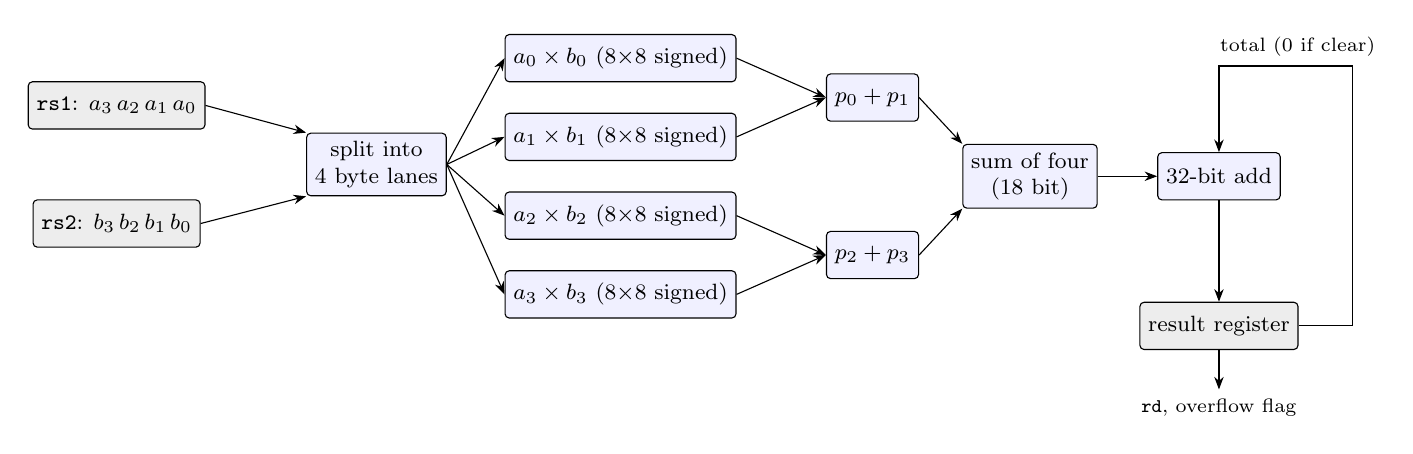
\begin{tikzpicture}[x=1cm,y=1cm,font=\footnotesize,
  box/.style={draw,rounded corners=1.5pt,minimum height=0.6cm,inner sep=3pt,fill=blue!6},
  reg/.style={draw,rounded corners=1.5pt,minimum height=0.6cm,inner sep=3pt,fill=gray!14},
  arr/.style={-{Stealth[length=1.6mm]}}]
\node[reg] (rs1) at (0,2.4) {\texttt{rs1}: $a_3\,a_2\,a_1\,a_0$};
\node[reg] (rs2) at (0,0.9) {\texttt{rs2}: $b_3\,b_2\,b_1\,b_0$};
\node[box,align=center] (lanes) at (3.3,1.65) {split into\\4 byte lanes};
\draw[arr] (rs1.east) -- (lanes.north west);
\draw[arr] (rs2.east) -- (lanes.south west);
\foreach \i/\y in {0/3.0,1/2.0,2/1.0,3/0.0}{
  \node[box] (m\i) at (6.4,\y) {$a_\i\times b_\i$ (8$\times$8 signed)};
  \draw[arr] (lanes.east) -- (m\i.west);
}
\node[box] (s01) at (9.6,2.5) {$p_0+p_1$};
\node[box] (s23) at (9.6,0.5) {$p_2+p_3$};
\draw[arr] (m0.east) -- (s01.west);
\draw[arr] (m1.east) -- (s01.west);
\draw[arr] (m2.east) -- (s23.west);
\draw[arr] (m3.east) -- (s23.west);
\node[box,align=center] (s4) at (11.6,1.5) {sum of four\\(18 bit)};
\draw[arr] (s01.east) -- (s4.north west);
\draw[arr] (s23.east) -- (s4.south west);
\node[box,align=center] (add) at (14.0,1.5) {32-bit add};
\draw[arr] (s4.east) -- (add.west);
\node[reg,align=center] (res) at (14.0,-0.4) {result register};
\draw[arr] (add.south) -- (res.north);
\draw[arr] (res.east) -- (15.7,-0.4) -- (15.7,2.9) -- (14.0,2.9) -- (add.north);
\node[font=\scriptsize,anchor=south] at (15.0,2.9) {total (0 if clear)};
\draw[arr] (res.south) -- ++(0,-0.5) node[below,font=\scriptsize] {\texttt{rd}, overflow flag};
\end{tikzpicture}}
\caption{Datapath of the unit. The running total is fed back from the result register, so the accumulating instructions need no third register read.}
\label{fig:datapath}
\end{figure}

The four instructions are R-type in opcode \texttt{0x0B} (\texttt{custom-0}) with \texttt{funct3} = 0:

\begin{center}
\begin{tabular}{@{}llp{9.3cm}@{}}
\toprule
Instruction & \texttt{funct7} & Operation \\
\midrule
\simd{mac}     & \texttt{0000000} & \texttt{rd = rd + dot4(rs1, rs2)} \\
\simd{mac\_clr} & \texttt{0000001} & \texttt{rd = dot4(rs1, rs2)} \\
\simd{macc}    & \texttt{0000010} & \texttt{total = total + dot4(rs1, rs2); rd = total} \\
\simd{macz}    & \texttt{0000011} & \texttt{total = dot4(rs1, rs2); rd = total} \\
\bottomrule
\end{tabular}
\end{center}

\begin{figure}[htbp]
\centering
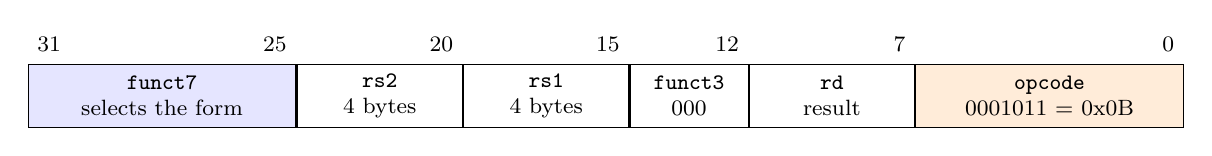
\begin{tikzpicture}[font=\footnotesize,
  f/.style={draw,minimum height=8mm,align=center,inner sep=0pt}]
\node[f,minimum width=34mm,fill=blue!10] (a) at (0,0) {\texttt{funct7}\\selects the form};
\node[f,minimum width=21mm,right=0pt of a] (b) {\texttt{rs2}\\4 bytes};
\node[f,minimum width=21mm,right=0pt of b] (c) {\texttt{rs1}\\4 bytes};
\node[f,minimum width=15mm,right=0pt of c] (d) {\texttt{funct3}\\000};
\node[f,minimum width=21mm,right=0pt of d] (e) {\texttt{rd}\\result};
\node[f,minimum width=34mm,right=0pt of e,fill=orange!15] (g) {\texttt{opcode}\\0001011 = 0x0B};

\node[above=1pt of a.north west,anchor=south west] {31};
\node[above=1pt of a.north east,anchor=south east] {25};
\node[above=1pt of b.north east,anchor=south east] {20};
\node[above=1pt of c.north east,anchor=south east] {15};
\node[above=1pt of d.north east,anchor=south east] {12};
\node[above=1pt of e.north east,anchor=south east] {7};
\node[above=1pt of g.north east,anchor=south east] {0};
\end{tikzpicture}
\caption{Instruction format. The four instructions differ only in \texttt{funct7}, so one decoder check on the opcode and \texttt{funct3} is enough to route them to the unit.}
\label{fig:encoding}
\end{figure}

\textbf{Two read ports.} The form \simd{mac} reads three registers (\texttt{rs1}, \texttt{rs2} and the old \texttt{rd}), but the PCPI port of PicoRV32 passes only two. \simd{macc} and \simd{macz} keep the running total inside the unit instead. Measured on an iCE40 UP5K, this change cost one LUT (84 to 85) and no clock speed. The total survives other instructions between MAC instructions but is not saved on a context switch, which suits bare-metal firmware.

\textbf{Software.} Firmware emits the instructions with the standard \texttt{.insn} assembler directive, so the compiler is not modified. Spike runs them through an extension library with the same semantics as the Verilog.

\subsection{Integration with PicoRV32}
The unit sits behind a decoder for \texttt{custom-0} and is attached through PCPI. The adapter issues the instruction and returns the result one cycle later. A custom instruction is therefore not free of overhead: in the trace of Section~\ref{sec:trace} it takes 4.0 cycles, which is why the speed-up in cycles is slightly below the speed-up in instructions.

\subsection{Firmware versions}
The firmware runs the same network five ways, and only the inner loop of the dot product differs:

\begin{enumerate}[label=(\arabic*)]
\item scalar, plain loop: byte loads and \texttt{mul};
\item scalar, loop unrolled 16 times;
\item \simd{mac\_clr} with an \texttt{add} to carry the total;
\item \simd{macz}/\simd{macc}, total kept in the unit;
\item as (4), loop unrolled 8 times.
\end{enumerate}

The \emph{fair comparison} is (2) against (5). Unrolling helps both sides, so only the hardware differs. Comparing (5) with (1) gives 7.65$\times$ in cycles, but that number mixes the effect of the hardware with the effect of unrolling, and I do not use it as the headline.

\section{Verification}
Each stage is checked against the one before it, and each check is shown to be able to fail (Table~\ref{tab:verify}).

\begin{table}[htbp]
\centering
\caption{Verification runs. All counts are from the repository's recorded results.}
\label{tab:verify}
\small
\begin{tabular}{@{}p{6.6cm}p{3.9cm}p{5.4cm}@{}}
\toprule
Check & Size & Result \\
\midrule
Unit RTL against the C++ golden model (real test image) & 25,088 vectors (128 neurons $\times$ 196 chunks) & 0 mismatches \\
Custom-0 wrapper as an instruction stream, with random data on \texttt{rd} and idle cycles & 25,088 instructions, 3,115 idle cycles & 0 mismatches \\
Custom-instruction self-test on Spike & 19,005 checks & all pass \\
Custom-instruction self-test on the PicoRV32 SoC & 14,005 checks & all pass \\
Firmware outputs against the C++ engine, 5 versions & 10 images (one per digit) & bit-exact; Spike and RTL instruction counts equal \\
\bottomrule
\end{tabular}
\end{table}

\textbf{The checks can fail.} Flipping one adder in the RTL gives 24,444 mismatches. Breaking the accumulator feedback, or making \simd{macz} forget to clear, gives about 24,900 mismatches each. A core built without the unit stops on the first custom instruction, and continuous integration requires that, so the self-test is known to be able to fail. A one-bit fault injected into the adapter also fails the self-test.

\begin{figure}[htbp]
\centering
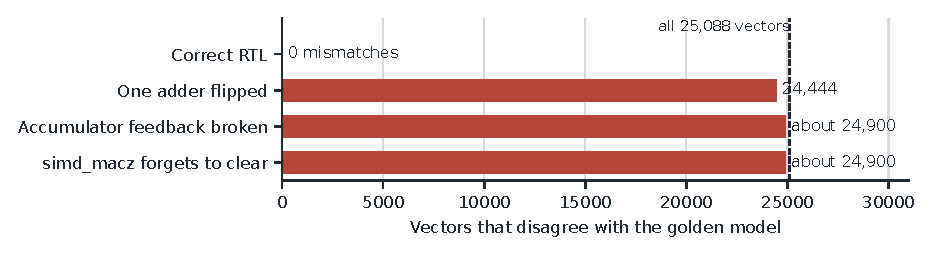
\includegraphics[width=0.88\textwidth]{figures/fig_faults.pdf}
\caption{The check is able to fail. Each faulty version of the RTL is compared with the golden model on the same 25,088 vectors.}
\label{fig:faults}
\end{figure}

\textbf{Continuous integration.} On every push, GitHub Actions rebuilds the engine, re-runs the RTL co-simulation, the Spike run and the whole-SoC simulation, compares each result with the recorded file, and fails if they differ. The wait-state sweep and the area and clock numbers depend on tool builds and take longer, so they are recorded by hand and are not re-checked there; the zero-wait row of the sweep is cross-checked against the SoC run.

\section{Evaluation}
\subsection{Results at a glance}
\begin{figure}[htbp]
\centering
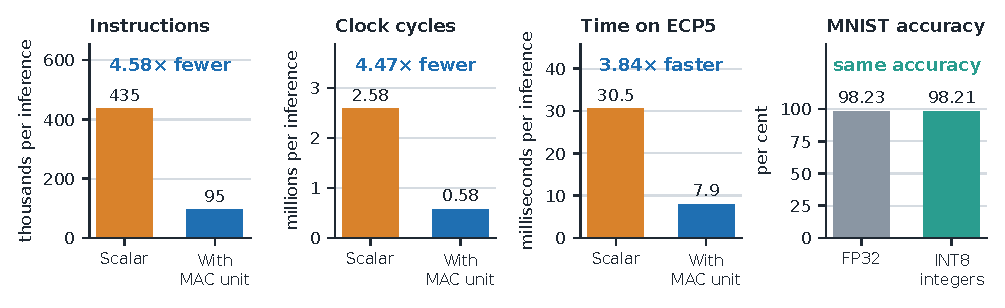
\includegraphics[width=\textwidth]{figures/fig_summary.pdf}
\caption{Key results. Scalar is the unrolled scalar loop, and ``with MAC unit'' is the unrolled loop that uses the custom instructions. Time is estimated from simulated cycles and the best place-and-route clock speed on an ECP5 FPGA.}
\label{fig:summary}
\end{figure}

\subsection{Method}
\textbf{Cycles.} The whole SoC (PicoRV32, the adapter, the unit and a memory model) is compiled from Verilog to C++ with Yosys CXXRTL and simulated cycle by cycle. The firmware reads \texttt{rdcycle}. Memory is a flat array that answers after a fixed number of wait states. PicoRV32 prefetches speculatively, so instruction boundaries in the trace are reconstructed from changes of the program counter and not from bus fetches. \textbf{Instructions} are counted in Spike and, separately, in the RTL; the two agree for every version.

\textbf{Area and clock speed.} Yosys \texttt{synth\_ecp5} and \texttt{synth\_ice40 -dsp}; place-and-route with nextpnr-ecp5 for an LFE5U-25F (CABGA256), three placement seeds. iCE40 numbers are synthesis only, because the SoC has more pins than the UP5K package offers and the HX8K has no DSP blocks.

\subsection{Accuracy}
Activation scales are calibrated on 2,000 training images and the 10,000 test images are used only for the final figures. The INT8 result was cross-checked with an independent NumPy implementation of the same integer pipeline, which also gives 98.21\%. INT8 and FP32 predict the same class on 99.84\% of the test images (9,984 of 10,000).

\begin{center}
\begin{tabular}{@{}lr@{}}
\toprule
Configuration & MNIST test accuracy \\
\midrule
FP32 reference & 98.23\% \\
INT8 weights, FP32 activations & 98.23\% \\
INT8 end to end, integer-only (main configuration) & 98.21\% \\
\bottomrule
\end{tabular}
\end{center}

\subsection{Instructions and clock cycles}
\begin{table}[htbp]
\centering
\caption{One inference, no wait states. Instructions are from Spike and agree with the RTL; cycles are from the RTL simulation.}
\label{tab:cycles}
\small
\begin{tabular}{@{}lrrr@{}}
\toprule
Version & Instructions & Clock cycles & Cycles per instruction \\
\midrule
(1) Scalar, plain loop & 822,232 & 4,416,182 & 5.4 \\
(2) Scalar, unrolled & 435,282 & 2,583,289 & 5.9 \\
(3) \simd{mac\_clr} + \texttt{add} & 187,598 & 1,014,656 & 5.4 \\
(4) \simd{macz}/\simd{macc} & 161,500 & 908,620 & 5.6 \\
(5) as (4), unrolled & 95,120 & 577,451 & 6.1 \\
\bottomrule
\end{tabular}
\end{table}

The fair speed-up (2) against (5) is \textbf{4.58$\times$ in instructions} and \textbf{4.47$\times$ in clock cycles} (Figure~\ref{fig:versions}). It is lower in cycles because the MAC loop averages 6.1 cycles per instruction against 5.9 for the scalar loop. Running the scalar code on the core with the unit removed takes exactly the same 4,416,182 cycles, so the unit does not slow down ordinary code.

\begin{figure}[htbp]
\centering
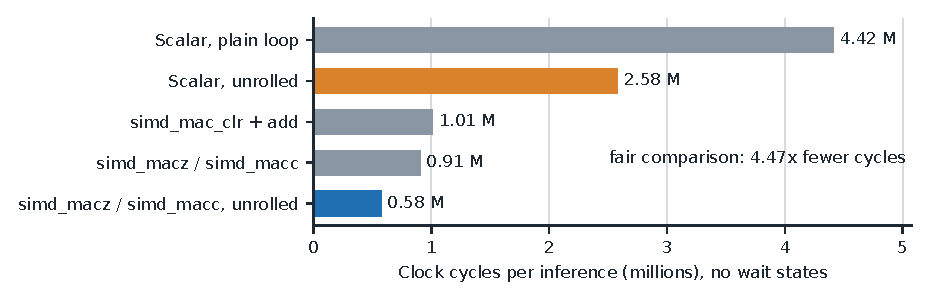
\includegraphics[width=0.84\textwidth]{figures/fig_versions.pdf}
\caption{Clock cycles per inference for the five versions. The fair comparison is the two unrolled versions (orange and blue).}
\label{fig:versions}
\end{figure}

\begin{figure}[htbp]
\centering
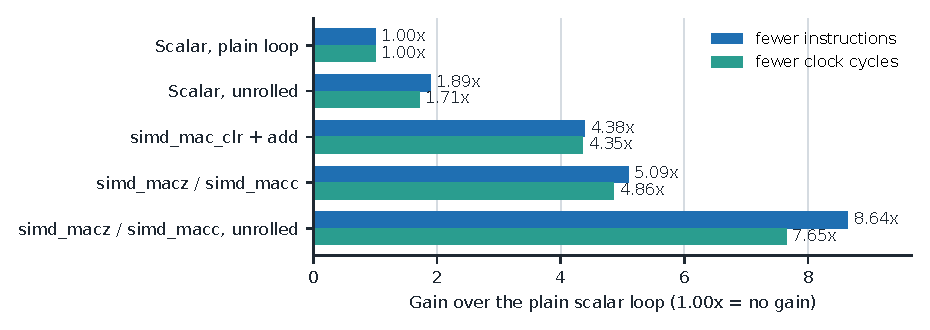
\includegraphics[width=0.88\textwidth]{figures/fig_gain.pdf}
\caption{The same five versions as a gain over the plain scalar loop. Unrolling alone gives 1.71$\times$ in cycles; the custom instructions on top give a further 4.47$\times$.}
\label{fig:gain}
\end{figure}

\subsection{Slower memory}
The testbench delays every memory reply. PicoRV32 has no cache and fetches every instruction from memory, so memory time grows with the instruction count. Cutting the instructions by about 4.6$\times$ cuts memory time by about as much, and the speed-up stays nearly flat (Figure~\ref{fig:wait}): 4.47$\times$ with none and 4.27$\times$ with 16 wait states. A core with caches or tightly coupled memory would behave differently; that was not measured.

\begin{figure}[htbp]
\centering
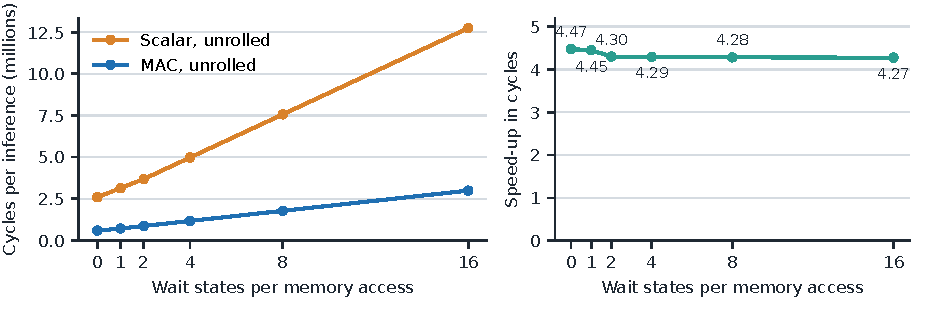
\includegraphics[width=0.88\textwidth]{figures/fig_waitstates.pdf}
\caption{Unrolled versions with 0 to 16 wait states per memory access (image 0). Left: cycles per inference. Right: speed-up.}
\label{fig:wait}
\end{figure}

\subsection{Area, clock speed and time}
\begin{table}[htbp]
\centering
\caption{Area and clock speed. ECP5: after place-and-route, three seeds. iCE40: synthesis only.}
\label{tab:area}
\small
\begin{tabular}{@{}lrrrr@{}}
\toprule
 & LUT4 & Flip-flops & DSP blocks & Fmax \\
\midrule
Core without the unit, ECP5 & 1,942 & 924 & 4 & 82.1 to 84.8 MHz \\
Core with the unit, ECP5 & 2,487 & 958 & 8 & 69.7 to 72.8 MHz \\
MAC unit alone, ECP5 & 419 & 34 & 4 & \\
Core without the unit, iCE40 & 2,734 & 931 & 4 & \\
Core with the unit, iCE40 & 2,785 & 965 & 8 & \\
MAC unit alone, iCE40 & 76 & 34 & 4 & \\
\bottomrule
\end{tabular}
\end{table}

\begin{figure}[htbp]
\centering
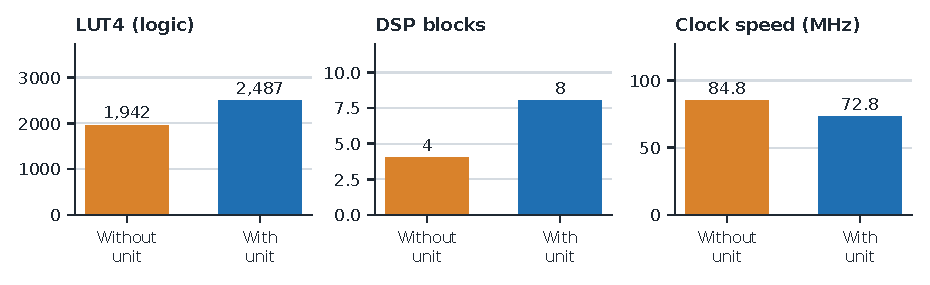
\includegraphics[width=0.88\textwidth]{figures/fig_cost.pdf}
\caption{Cost of the unit on ECP5: the whole SoC without and with it (after place-and-route, best of three seeds for clock speed).}
\label{fig:cost}
\end{figure}

The unit costs 34 flip-flops and 4 DSP blocks on both devices. LUTs differ a lot: on iCE40 each \texttt{SB\_MAC16} also adds and accumulates, while on ECP5 the multipliers have no accumulator, so the adder tree and the 32-bit total go into logic. On the full ECP5 SoC the difference is 545 LUT4, more than the 419 of the unit alone; I did not separate the rest.

The unit lowers the clock speed by about 12~MHz (14\%, best of three seeds), because the multiply, the adder tree and the accumulation happen in one cycle and that path is now the longest. At those speeds one inference takes about 30.5~ms with the unrolled scalar loop (2,583,289 cycles at 84.8~MHz) and about 7.9~ms with the unit (577,451 cycles at 72.8~MHz). That is \textbf{about 3.8$\times$ faster in time}, not 4.47$\times$. The estimate uses the best seed of each design and ignores the memory system.

\subsection{Where the cycles go}
\label{sec:trace}
I recorded layer 1, neuron 0 of image 0 (784 multiply-accumulates) from the RTL simulation, instruction by instruction, once for the unrolled scalar loop and once for the unrolled MAC loop. Each instruction is charged the cycles between one change of the program counter and the next.

\begin{figure}[htbp]
\centering
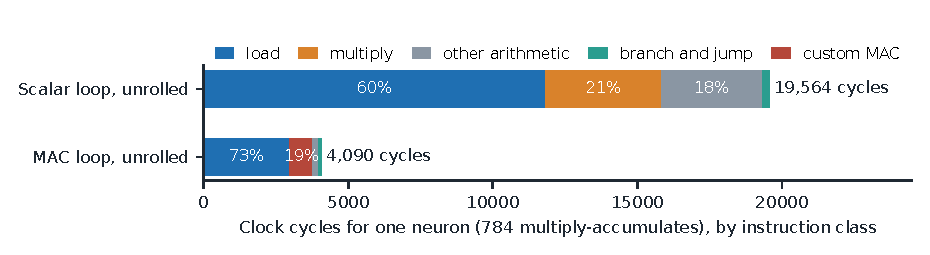
\includegraphics[width=0.9\textwidth]{figures/fig_neuron.pdf}
\caption{Cycles of one neuron by instruction class.}
\label{fig:neuron}
\end{figure}

\begin{table}[htbp]
\centering
\caption{One neuron, by instruction class: instructions / cycles (average cycles per instruction).}
\label{tab:neuron}
\small
\begin{tabular}{@{}lrrrr@{}}
\toprule
Class & \multicolumn{2}{c}{Scalar, unrolled} & \multicolumn{2}{c}{MAC, unrolled} \\
\cmidrule(lr){2-3}\cmidrule(lr){4-5}
 & Instr./cycles & Cyc./instr. & Instr./cycles & Cyc./instr. \\
\midrule
Load & 1,568 / 11,807 & 7.5 & 391 / 2,981 & 7.6 \\
Multiply & 784 / 4,018 & 5.1 & --- & --- \\
Custom MAC & --- & --- & 196 / 784 & 4.0 \\
Other arithmetic & 885 / 3,490 & 3.9 & 50 / 200 & 4.0 \\
Branch and jump & 50 / 249 & 5.0 & 26 / 125 & 4.8 \\
\midrule
Total & 3,287 / 19,564 & 6.0 & 663 / 4,090 & 6.2 \\
\bottomrule
\end{tabular}
\end{table}

For this neuron the gain is 4.96$\times$ in instructions and 4.78$\times$ in cycles. The whole inference gives a smaller 4.47$\times$; I attribute the difference to work outside the dot product (setup and requantisation for each neuron) and to the shorter second layer, but I did not trace those parts.

The accelerated loop is dominated by memory access, not by the unit: \textbf{73\% of its cycles are loads and 19\% are the custom instruction}. Each custom instruction needs two 32-bit loads, one of four activation bytes and one of four weight bytes (391 loads for 196 custom instructions). If the custom instructions took no cycles at all, the neuron would still need 3,306 cycles, so the gain could rise only to about 5.9$\times$ (an upper bound computed from the table, not a measurement). The next gain therefore has to come from loading fewer operands, for example by reusing an activation word across several neurons, and not from a faster multiplier. This also explains why a small cache or tightly coupled memory, which makes loads cheaper, could change the result.

\section{Limitations}
These are things I did not measure or did not do:
\begin{itemize}
\item Memory is a flat array with a fixed number of wait states: no cache, no real DRAM or flash timing.
\item The baseline core has the fast multiplier. With PicoRV32's small serial multiplier the scalar code would be slower and the gain larger; I did not run it.
\item Xilinx 7-series timing and any ASIC flow were not run. iCE40 numbers for the full SoC are synthesis only.
\item Clock speeds come from nextpnr on one device family and three placement seeds. They are not silicon measurements, and the 3.8$\times$ estimate in time inherits that.
\item Both sides are compiled C at \texttt{-O2} (xPack RISC-V GCC 14.2.0). Hand-written assembly on either side was not tried.
\item One network (a 784-128-10 MLP) on one dataset; other layer shapes, such as convolutions, were not run.
\item Power was not measured.
\end{itemize}

\section{Conclusion and future work}
A 4-lane INT8 MAC unit with four instructions in the \texttt{custom-0} opcode gives 4.47$\times$ fewer clock cycles per inference than an equally unrolled scalar loop on PicoRV32, and about 3.8$\times$ less time on an ECP5 FPGA after the unit's cost in clock speed. The result holds when memory gets slower, the integer-only network loses 0.02 percentage points of accuracy against FP32, and every number is produced by a command in the repository and checked in continuous integration. The cycle trace shows where the remaining time is: in loading operands.

Next steps, in the order I would do them: (i) run the baseline with the serial multiplier, which removes the largest open limit; (ii) reduce operand loads by reusing activations across neurons, which needs more than one accumulator in the unit; (iii) pipeline the adder tree to recover clock speed at the price of one more cycle per instruction; (iv) measure with a cache or tightly coupled memory; (v) try other layer shapes.

\paragraph{Availability.} Code, firmware, Verilog, recorded results and the figure script are at \url{https://github.com/sajedulislam5840/riscv-edge-ai}. \texttt{BENCHMARKS.md} lists how every number is measured, and the \texttt{README.md} gives the commands to reproduce it. A replay of the trace is at \url{https://sajedulislam5840.github.io/riscv-edge-ai/}.

\begin{thebibliography}{9}\small
\bibitem{jacob2018} B.~Jacob, S.~Kligys, B.~Chen, M.~Zhu, M.~Tang, A.~Howard, H.~Adam and D.~Kalenichenko, ``Quantization and training of neural networks for efficient integer-arithmetic-only inference,'' in \emph{Proc.\ IEEE/CVF Conf.\ on Computer Vision and Pattern Recognition (CVPR)}, 2018, pp.~2704--2713.
\bibitem{lai2018} L.~Lai, N.~Suda and V.~Chandra, ``CMSIS-NN: Efficient neural network kernels for Arm Cortex-M CPUs,'' arXiv:1801.06601, 2018.
\bibitem{hauser} J.~Hauser, ``Proposed instructions for the RISC-V Base P extension,'' draft proposal, not an official RISC-V document, version 012, 2024. \url{https://jhauser.us/RISCV/ext-P/RVP-baseInstrs-012.pdf}
\bibitem{prakash2023} S.~Prakash, T.~Callahan, J.~Bushagour, C.~Banbury, A.~V.~Green, P.~Warden, T.~Ansell and V.~J.~Reddi, ``CFU Playground: Full-stack open-source framework for tiny machine learning (tinyML) acceleration on FPGAs,'' in \emph{Proc.\ IEEE Int.\ Symp.\ on Performance Analysis of Systems and Software (ISPASS)}, 2023, pp.~157--167.
\bibitem{picorv32} C.~Wolf, ``PicoRV32: a size-optimized RISC-V CPU,'' \url{https://github.com/YosysHQ/picorv32}.
\end{thebibliography}

\end{document}
